\section{Results}
In this section we will show the results that we obtainfor the three materials
and we will compare them with ONELDANT\cite{cepxs}. ONELDANT is a code which
solve the BFP equation in one dimension using the cross sections generated by
CEPXS. The code that we are developing is three dimensional. To compare the 
results produced by the two codes, we use the same spatial discretization 
(linear discontinuous finite element) and equivalent angular discretization 
(Gauss-Legendre for ONELDANT and Gauss-Legendre-Chebyshev for our code). 
The number of cells is the same in the direction of comparison. The only 
difference is in the output. ONELDANT gives only the average dose on a cell and 
that our code give the value at a given point. To compare the value of the dose 
at a given point, we will interpolate the value given by ONELDANT.

\subsection{Water}
For this example, we are using a $S_{12}$ Galerkin-Legendre-Chebyshev
quadrature. The medium is 5 cm thick and there is an incoming flux of
photons. The direction of the flux is chosen to be the most normal direction
of the quadrature and the value of the flux is 1 $\frac{n}{cm^2s}$. The source 
of photons has an energy of 20 MeV and we use a cut-off energy of 0.01 MeV. 
Every particle that has an energy lower than 0.01 MeV is assumed to depose 
all its energy without moving further.\\
In the next table, we show the dose computed every centimeter using a
different scattering \hbox{order :}
\begin{table}[H]
\begin{center}
\caption{Dose in $\frac{MeV}{g}$ for different scattering orders}
\begin{tabular}{|c|c|c|c|c|c|c|}
\hline
Position & ONELDANT & order = 13 & order = 11 & order = 9 & order = 7 & order = 5 \\
\hline
0 & 4.92645e-3 &  &  &  &  &  \\
1 & 5.68274e-2 &  &  &  &  &  \\
2 & 1.05076e-1 &  &  &  &  &  \\
3 & 1.47528e-1 &  &  &  &  &  \\
4 & 1.82864e-1 &  &  &  &  &  \\
5 & 1.85907e-1 &  &  &  &  &  \\
\hline
\end{tabular}
\end{center}
\end{table}     

\subsection{Aluminium}
The setup of this problem, is the same as that of the previous one but the medium is
composed of aluminium. In the following table, we show the dose computed every 
centimeter using a different scattering order :
\begin{table}[H]
\begin{center}
\caption{Dose in $\frac{MeV}{g}$ for different scattering orders}
\begin{tabular}{|c|c|c|c|c|c|c|}
\hline
Position & ONELDANT & order = 13 & order = 11 & order = 9 & order = 7 & order = 5 \\
\hline
0 & 0.015003 & 0.0146404 & 0.0146402 & 0.0141156 & 0.0166718 & 0.0087276 \\
1 & 0.169908 & 0.1697907 & 0.1697890 & 0.1698012 & 0.1695422 & 0.1728969 \\
2 & 0.275425 & 0.2752749 & 0.2752729 & 0.2753298 & 0.2742052 & 0.2775113 \\
3 & 0.316307 & 0.3161310 & 0.3161307 & 0.3165279 & 0.3145572 & 0.3199176 \\
4 & 0.312283 & 0.3120572 & 0.3120566 & 0.3125514 & 0.3104412 & 0.3153226 \\
5 & 0.233048 & 0.2087631 & 0.2087634 & 0.2094064 & 0.2061794 & 0.2154810 \\
\hline
\end{tabular}
\end{center}
\end{table}     
The agreement between ONELDANT and our code using the full order is excellent.
The differences on the border of the domain are larger due to the fact that
the dose varies quickly and thus, the interpolation used to find the value at
a given point by ONELDANT is not very accurate.\\ 
We can see that if we except the border of the domain, the results obtained by
using a $P_5$ order for the scattering are very close to the results using the
full order. The reason is that the high order moments are very small. Below,
we show several moments, for different groups. The abscissa is the distance in
centimeter and the ordinate is the value of the flux in $\frac{particle}{cm^2
s}$.
\begin{figure}[H]
\begin{minipage}[b]{0.45\linewidth}
\centering
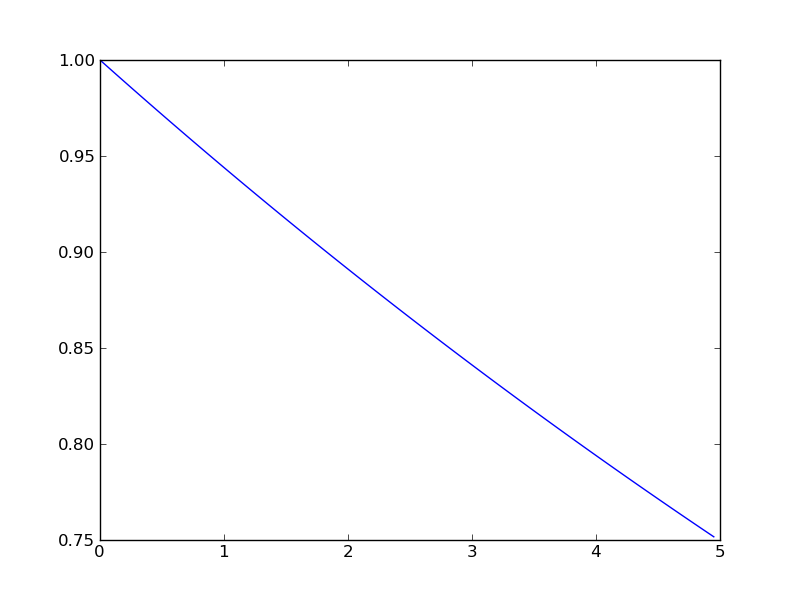
\includegraphics[width=\linewidth]{./images/al/group_0_moment_0}
\caption{Scalar flux for the first group of photons}
\end{minipage}
\hspace{0.5cm}
\begin{minipage}[b]{0.45\linewidth}
\centering
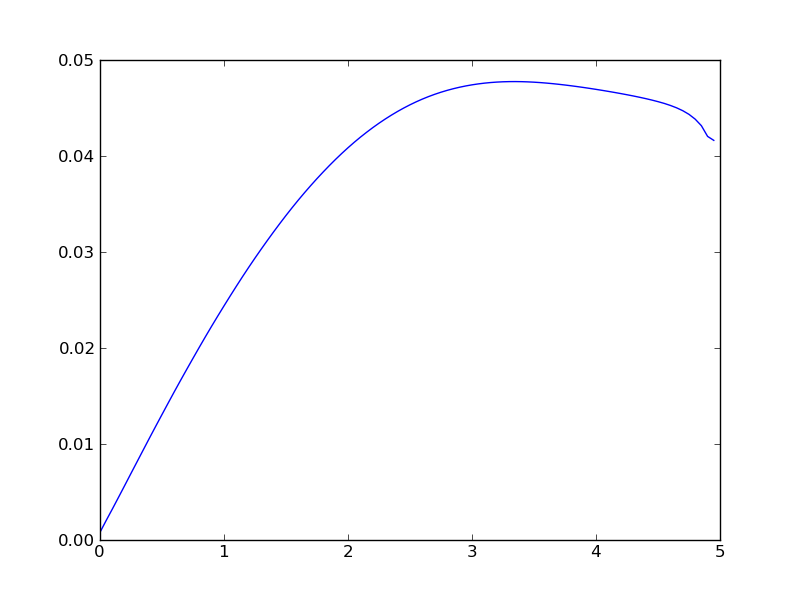
\includegraphics[width=\linewidth]{./images/al/group_39_moment_0}
\caption{Scalar flux for the last group of electrons}
\end{minipage}
\end{figure}

\begin{figure}[H]
\begin{minipage}[b]{0.45\linewidth}
\centering
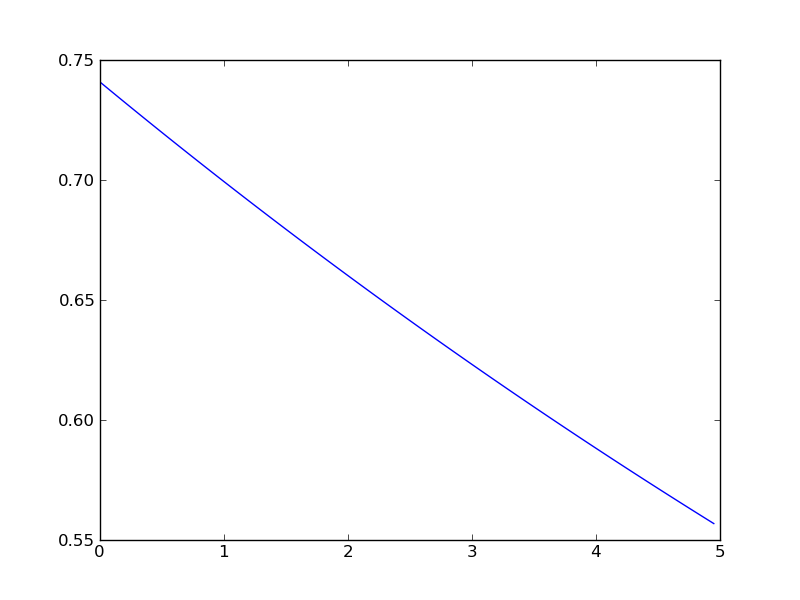
\includegraphics[width=\linewidth]{./images/al/group_0_moment_30}
\caption{Moment $P_5^0$ of the flux for the first group of photons}
\end{minipage}
\hspace{0.5cm}
\begin{minipage}[b]{0.45\linewidth}
\centering
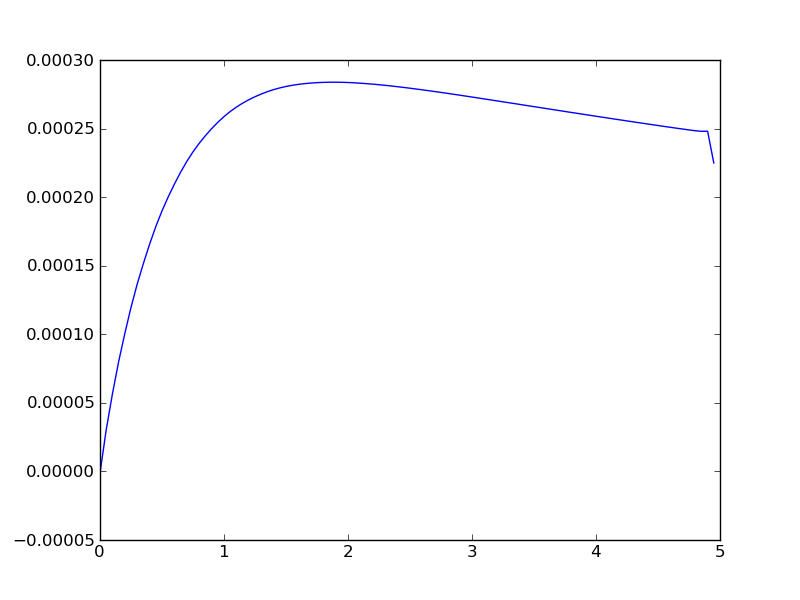
\includegraphics[width=\linewidth]{./images/al/group_39_moment_30}
\caption{Moment $P_5^0$ of the flux for the last group of electrons}
\end{minipage}
\end{figure}

\begin{figure}[H]
\begin{minipage}[b]{0.45\linewidth}
\centering
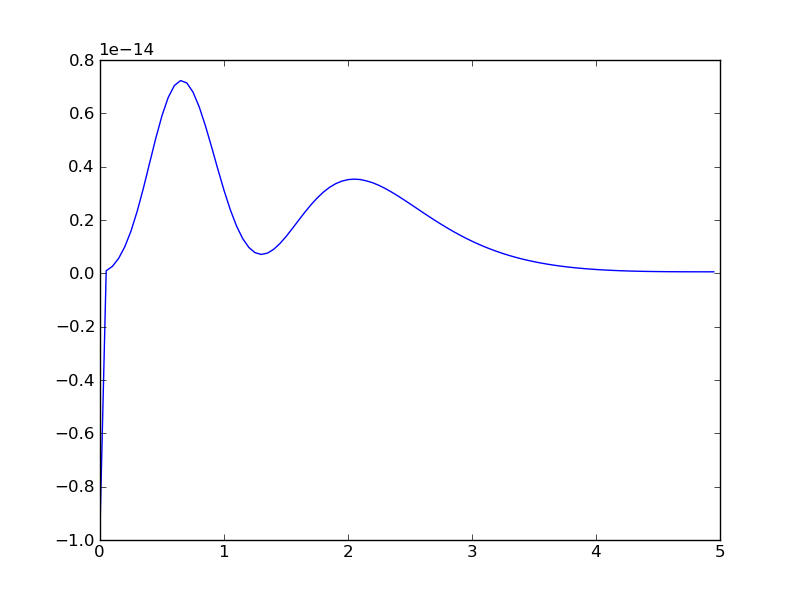
\includegraphics[width=\linewidth]{./images/al/group_0_moment_142}
\caption{Moment $P_{11}^0$ of the flux for the first group of photons}
\end{minipage}
\hspace{0.5cm}
\begin{minipage}[b]{0.45\linewidth}
\centering
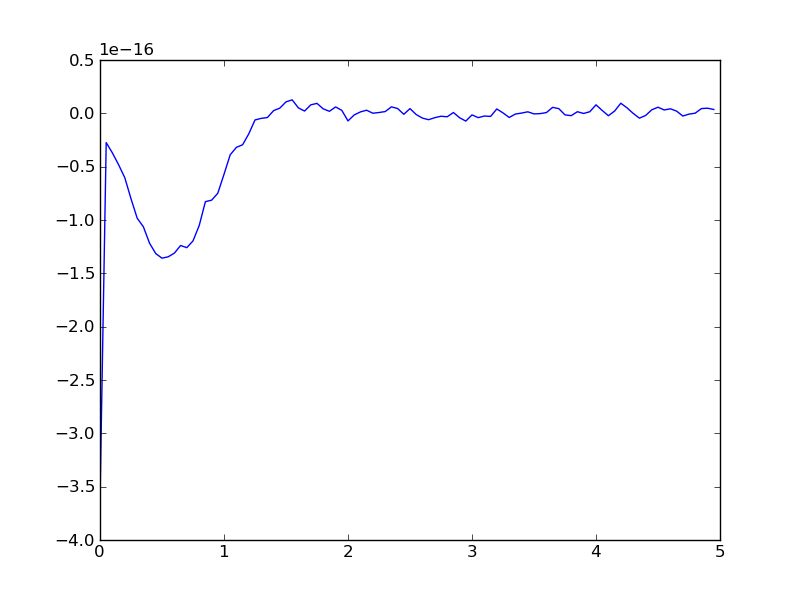
\includegraphics[width=\linewidth]{./images/al/group_39_moment_142}
\caption{Moment $P_5^0$ of the flux for the last group of electrons}
\end{minipage}
\end{figure}

\subsection{Gold}
The setup of this problem is the same as that of the same the others but now 
the medium is made of gold. In the next table, 
we show the dose computed every centimeter using a different scattering order :
\begin{table}[H]
\begin{center}
\caption{Dose in $\frac{MeV}{g}$ for different scattering orders}
\begin{tabular}{|c|c|c|c|c|c|c|}
\hline
Position & ONELDANT & order = 13 & order = 11 & order = 9 & order = 7 & order = 5 \\
\hline
0 & 0.11675 &  &  & 0.097155 & 0.097073 & 0.097326 \\
1 & 0.41799 &  &  & 0.420871 & 0.420988 & 0.421102 \\
2 & 0.16284 &  &  & 0.164946 & 0.165017 & 0.164605 \\
3 & 0.06407 &  &  & 0.065300 & 0.065292 & 0.065214 \\
4 & 0.02566 &  &  & 0.026304 & 0.026295 & 0.026318 \\
5 & 0.00847 &  &  & 0.006083 & 0.006075 & 0.006112 \\
\hline
\end{tabular}
\end{center}
\end{table}     
